\section{Background Research}
% The background section must outline the necessary background to the project,
% stating how it is important for the project work. For example: survey of related
% literature, analysis of competing products, technical specifications of hardware
% or software standards, electronic components, necessary software tools,
% background theory. The contents of this section will vary for different
% projects, and in many cases the background reading will have been completed –
% but if not you should be in a position to list what remains to be done (e.g. a
% set of research papers to read and understand). A good benchmark of progress
% here is that you have accumulated (though may not yet have read) at least 20
% references to background material. In projects which have substantial background
% writing up your literature survey in the Interim Report will save time at the
% end of the project and allow this element of your final report to receive timely
% feedback from your supervisor so the final write-up can be improved.
% REVISIT: Better logic between serial and parallel operators. The project is
% REVISIT: mostly with parallel operators so limit the background for serial.

\subsection{On-line Arithmetic}
Traditional proposals to achieving a faster and more efficient arithmetic
operator have two common characteristics.
One, their order operation may be different depending on the operation itself.
A traditional adder, parallel or serial, generates its answers from the LSD to
the MSD.
A traditional divider design on the other hand, generates its answers from
the MSD to the LSD~\cite{Brent1}\cite{Srinivas1}.

Due to this inconsistency, arithmetic operators may be forced to compute
word-by-word, waiting for all digits to finish in the previous operator before
moving on to the next.~\cite{Zhao1}
This means if a divider follows an adder of the same width, the divider has to
wait until the adder complete its computation before it can start its own.

The other commonality of traditional designs is that their precisions are
specified design-time. Once built, a 32-bit adder always adds 32 bits together,
as the hardware is fixed at run-time.
A possible way of making it more efficient would be using SIMD
instructions~\cite{Duncan1}, trying to combine smaller operations into a larger
one that fits the hardware.
This requires more control circuits in the hardware, or a more complex compiler.

On-line arithmetic does not suffer from the first issue as it performs all
arithmetic operations with MSD first~\cite{Ercegovac1}.
Pipelining can be used with on-line arithmetic operators.
This means the output digit of an earlier operation can be fed into the next
operator before the earlier operation been fully complete.

\begin{figure}[H]
  \centering
  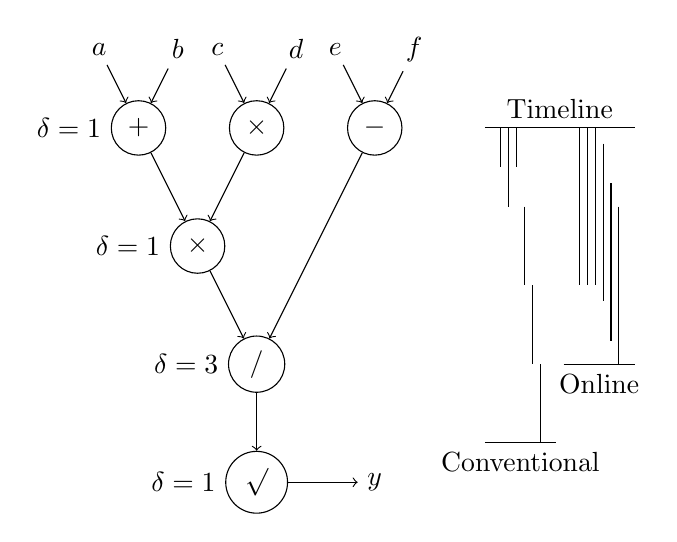
\begin{tikzpicture}
  \path
  (-0.5,5)   node(a) {$a$}
  (0.5,5)    node(b) {$b$}
  (1.0,5)    node(c) {$c$}
  (2,5)      node(d) {$d$}
  (2.5,5)    node(e) {$e$}
  (3.5,5)    node(f) {$f$}

  (0,4)      node[circle,draw,label=left:{$\delta=1$}](p1)  {$+$}
  (1.5,4)    node[circle,draw](p2)                          {$\times$}
  (3,4)      node[circle,draw](p3)                          {$-$}
  (0.75,2.5) node[circle,draw,label=left:{$\delta=1$}](p4)  {$\times$}
  (1.5,1)    node[circle,draw,label=left:{$\delta=3$}](p5)  {$/$}
  (1.5,-0.5) node[circle,draw,label=left:{$\delta=1$}](p6)  {$\surd$}

  (3,-0.5)   node(y) {$y$}
  ;

  \draw[->] (a) -- (p1);
  \draw[->] (b) -- (p1);
  \draw[->] (c) -- (p2);
  \draw[->] (d) -- (p2);
  \draw[->] (e) -- (p3);
  \draw[->] (f) -- (p3);

  \draw[->] (p1) -- (p4);
  \draw[->] (p2) -- (p4);
  \draw[->] (p3) -- (p5);
  \draw[->] (p4) -- (p5);
  \draw[->] (p5) -- (p6);

  \draw[->] (p6) -- (y);

  \draw (4.4,4) -- (6.3,4) node[midway,above]() {Timeline};;
  \draw (4.4,0) -- (5.3,0) node[midway,below]() {Conventional};
  \draw (5.4,1) -- (6.3,1) node[midway,below]() {Online};

  \draw (4.6,4) -- (4.6,3.5);
  \draw (4.7,4) -- (4.7,3);
  \draw (4.8,4) -- (4.8,3.5);
  \draw (4.9,3) -- (4.9,2);
  \draw (5.0,2) -- (5.0,1);
  \draw (5.1,1) -- (5.1,0);

  \draw (5.6,4) -- (5.6,2);
  \draw (5.7,4) -- (5.7,2);
  \draw (5.8,4) -- (5.8,2);
  \draw (5.9,3.8) -- (5.9,1.8);
  \draw (6.0,3.3) -- (6.0,1.3);
  \draw (6.1,3) -- (6.1,1);

\end{tikzpicture}
  \caption{Computing $y=\sqrt{(a+b)cd/(e-f)}$ with serial on-line
           operators~\cite{Ercegovac1}}
  \label{Online}
\end{figure}

As illustrated in figure~\ref{Online}, while each individual operation may
take longer than its conventional counterpart, on-line arithmetic could provide
a speed up if the operators are in serial.
Individually, on-line arithmetic also sacrifices in terms of memory.
As all computation are made MSD to LSD, the use of a redundant number system
is compulsory.
However, this redundancy also has its advantage in making the operators
scalable.
The time required per digit can be made independent of the length of the
operands.~\cite{Trivedi1}

A recent architecture proposal allows the precision of
on-line arithmetic to be controlled at run-time~\cite{Zhao1}.
Traditionally, this run-time control was restricted due to the parallel adders
present in the multipliers and dividers.
This architecture reuses a fixed-precision adder and stores residues in
on-chip RAM.
As such, a single piece of hardware can be used to calculate to any precision
limited only by the size of the on-chip RAM.

Another way that on-line arithmetic alleviates the problem of fixed precision
falls out directly from its MSD-first nature.
Suppose the output of a conventional ripple adder is sampled before
it has completed its operation.
In this case, the lower digits would have been completed, but the carry would
not have reached the higher ones.
This means the error on the result would be significant, as the top bits
were still undetermined~\cite{Shi1}.

However, if the output of a serial on-line adder is sampled before its
completion, the lower bits would be the undetermined ones.
This means the error of the operation would be small.
With overclocking, on-line arithmetic would fail gracefully, losing its
precision gradually from the lowest bits first.
Thus, it allows for a run-time trade-off between precision and
frequency~\cite{Shi2}.

\subsection{High radix Arithmetic}
Conventional designs of arithmetic operators use binary representations.
This was chosen four decades ago to maximise numerical accuracy per bit of data.
However, using a high radix representation system could yield better numerical
accuracy while reducing area cost of FPGAs.
For example, a hexadecimal floating-point adder has a 30\% smaller area-time
product than its binary counterpart, while still delivering equal worst-case
and better average-case numerical accuracy~\cite{Catanzaro1}.

However, the savings are not without trade-offs.
This trade-off can become unfavourable if the specification requires much I/O
and little computation~\cite{Whyte1}.
This is because the overhead of radix conversion would be significant.
It is also unwise to use high radix representations when the numbers are
unusually small, thus making the savings offered by the high radix
negligible~\cite{Catanzaro1}.

\subsection{High radix On-line Arithmetic}
Using high radix number representations for on-line arithmetic is a
relatively novel concept.
% REVISIT: can find problem with Lynch? his high radix looks weird
While there have been some research in this field~\cite{Lynch1}\cite{Lynch2},
this project takes a more direct approach by implementing custom operators
made for high radix on-line arithmetic on a FPGA.
This would allow for empirical results to be obtained, hopefully revealing
practical insights to the method.

As an potential extension to the project, optimising this exotic arithmetic
on a system level for popular FPGA accelerations such as neural networks would
be innovative as well.